% Adapt ME 537 HW05 P1--P3 to planar task velocities only.
% Shared layout adapted from the instructor's ME 537 homework sources.
\documentclass[12pt,letterpaper]{article}
\usepackage{mathptmx}
\usepackage[T1]{fontenc}
\usepackage{xcolor,amsmath,amssymb,xurl,listings,enumitem,tikz}
\textwidth=6.5in
\textheight=9in
\oddsidemargin=0in
\evensidemargin=0in
\topmargin=0in
\headheight=0in
\headsep=0in
\parskip=0.08in
\parindent=0in
\setlist[enumerate]{itemsep=0.04in,topsep=0.04in}
\lstset{basicstyle=\ttfamily\footnotesize,breaklines=true,columns=fullflexible,
keepspaces=true,showstringspaces=false,aboveskip=0.04in,belowskip=0.04in}
\newcommand{\R}[2]{{}^{#1}\!R_{#2}}
\newcommand{\T}[2]{{}^{#1}\!T_{#2}}
\newcommand{\courseheader}[2]{%
\setlength{\fboxrule}{2pt}\setlength{\fboxsep}{2mm}%
\fcolorbox{black}{white}{\parbox{\dimexpr\linewidth-2\fboxsep-2\fboxrule\relax}{\centering\textbf{Introduction to Robotics Homework \##1 -- Draft}}}\par
\textbf{#2}\par}
\newcommand{\conventions}{Use right-handed rotations, column vectors, radians,
and meters. $\R{A}{B}$ maps coordinates from frame $B$ into frame $A$;
$\T{A}{B}$ also includes the origin of $B$ expressed in $A$.}
\newcommand{\submission}{\textbf{Submit:} labeled hand derivations and sketches,
your changed Python source files, the requested numerical/visual evidence,
and an AI-use statement (including ``none'' if applicable). Show your reasoning
before using code to check hand calculations. Public checks are intentionally
limited. The instructor supplies the deadline and submission destination.}

\begin{document}
\courseheader{5}{Planar Jacobians and velocity interpretation}
\textbf{Schedule:} late week 4 through week 5, at most 1.5 weeks.
Build on HW02--HW04. The task is $[x,y,\psi]$, where $\psi$ is a single planar
heading and $\dot\psi=\omega_z$. No spatial orientation parameterization,
singularity analysis, or inverse-kinematics implementation is assigned.

\begin{enumerate}
\item \textbf{Derive a two-link planar Jacobian by hand.}
Two revolute joints rotate counterclockwise about upright Z. Link lengths
are $a_1,a_2$ and the second joint angle is relative to link 1.
\begin{enumerate}
\item Write the tip position $(x,y)$ and heading $\psi$ as functions of
$q_1,q_2$. Differentiate to obtain the $3\times2$ matrix mapping
$[\dot q_1,\dot q_2]^T$ to $[v_x,v_y,\omega_z]^T$.
\item For $a_1=0.4$ m, $a_2=0.3$ m, $q=[\pi/2,-\pi/2]$, and
$\dot q=[0.2,-0.1]$ rad/s, calculate the matrix and task velocity.
Sketch the tip's instantaneous XY motion and explain each output unit.
\end{enumerate}

\item \textbf{Implement a checked planar Jacobian.}
In \path{src/intro_robotics/kinematics.py}, complete
\texttt{SerialArm.jacob\_planar}. The provided geometry check permits
upright revolute axes and in-plane prismatic axes in the selected reference.
For joint $i$, let $\hat u_i$ be its unit axis in that reference, $p_i$ its origin,
and $p_e$ the selected tip position. Use the geometric column rules:
\[
J_i=\begin{cases}
\begin{bmatrix}(\hat u_i\times(p_e-p_i))_x\\(\hat u_i\times(p_e-p_i))_y\\(\hat u_i)_z\end{bmatrix},
&\text{revolute},\\[4pt]
\begin{bmatrix}(\hat u_i)_x\\(\hat u_i)_y\\0\end{bmatrix},&\text{prismatic}.
\end{cases}
\]
\begin{enumerate}
\item Use \texttt{joint\_frames(q)} to locate physical joints and rotate
each stored local axis into the reference frame. Do not assume every stored
axis is local Z. Return exactly three rows and one column per joint.
\item Preserve the provided \texttt{base}/\texttt{tip} options and scope
check. Run:
\begin{lstlisting}
python -m homework.hw05.hw05_planar_jacobian
\end{lstlisting}
Compare your two-link output with problem 1 and inspect the provided slider arm.
\end{enumerate}
\end{enumerate}

\newpage
\begin{enumerate}[start=3]
\item \textbf{Interpret velocity for a three-joint arm.}
Use \texttt{planar\_arm()} with lengths $[0.4,0.3,0.2]$ m,
$q=[\pi/2,-\pi/2,\pi/2]$, and $\dot q=[0.2,-0.1,0.1]$ rad/s.
\begin{enumerate}
\item Calculate $J(q)$ and $J(q)\dot q$ using your code. Explain the physical
meaning of each column, including the upright angular-velocity row.
\item Compare $p(q+\dot q\Delta t)-p(q)$ with
$[v_x,v_y]^T\Delta t$ for $\Delta t=0.01$ s and $0.2$ s.
Report the two position-error norms. Why is the Jacobian approximation local?
\item Run the viewer with \texttt{--show}. Its purple XY arrow represents
velocity multiplied by 0.5 s. Explain its direction; it is not a planned
finite-time path. Optional: try a fourth planar joint and inspect the added column.
For an optional 3D view of individual joint contributions, run
\texttt{python -m homework.hw05.play\_velocity} and select the linear or
angular arrows in its Velocity tab.
\end{enumerate}

\item \textbf{A point before the last joint.}
In a three-link planar arm, point $C$ lies on link 2, at distance $a_c$ from
joint 2. Its orientation is attached to link 2, not the final tool.
\begin{center}
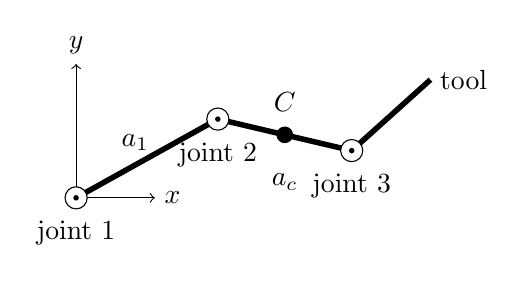
\begin{tikzpicture}[scale=1.0]
\draw[->] (0,0)--(1,0) node[right]{$x$};
\draw[->] (0,0)--(0,1.7) node[above]{$y$};
\draw[line width=2pt] (0,0)--(1.8,1)--(3.5,0.6)--(4.5,1.5);
\foreach \x/\y/\label in {0/0/1,1.8/1/2,3.5/0.6/3}{
\draw[fill=white] (\x,\y) circle (4pt);\fill (\x,\y) circle (1pt);
\node[below=5pt] at (\x,\y){joint \label};}
\fill (2.65,0.8) circle (3pt) node[above=5pt]{$C$};
\node at (0.75,0.7){$a_1$};\node at (2.65,0.2){$a_c$};
\node[right] at (4.5,1.5){tool};
\end{tikzpicture}
\end{center}
By hand, write $p_C(q)$, its link-2 heading, and the $3\times3$ Jacobian
for this point/frame. Explain the zero column physically. This derivation
is separate from the class method, which targets the final tip.

\item \textbf{Respect the scope of the velocity model.}
Try \texttt{spatial\_arm().fk([0,0,0])} and then its
\texttt{jacob\_planar([0,0,0])}. Report the explained scope error.
For the conveyor project, a separate actuator can lower/lift a pickup tool
with finite duration. Explain why that vertical motion is not another row
of this planar Jacobian. General spatial FK remains available.
\end{enumerate}

\submission
\end{document}
